\documentclass[../monografia.tex]{subfiles}

\begin{document}

\section{Requisitos Técnicos}

\subsection{Rede de Sensores}

Com base na pesquisa sobre os protocolos de rede mais adequados para aplicações de redes de sensores no contexto de internet das coisas, optamos por utilizar BLE em conjunto com Wi-fi. 

A fim de disponibilizar os dados coletados pelos diferentes sensores acerca do ambiente para posterior análise, se faz necessária uma conexão à Internet dos dispositivos desenvolvidos. Essa conexão será feita através do protocolo Wi-Fi, conectando o dispositivo em si a um ponto de acesso presente no ambiente analisado.

Como os dispositivos ficarão em escritórios, não seria ideal que todos eles ficassem conectados à rede Wi-Fi do local. Como mostrado na seção \ref{topologias-rede}, o protocolo Wi-Fi possui alto consumo energético, outro ponto negativo já que visamos alimentar os dispositivos com baterias. Dessa forma, o protocolo BLE será utilizado para interconectar os dispositivos, dado seu baixo consumo de energia, alta escalabilidade e alta taxa de transmissão de dados, quando comparado com as outras tecnologias apresentadas.

\subsection{Parâmetros de Medição}

Definimos as métricas de \textbf{qualidade do ambiente} com base nos níveis considerados saudáveis pela literatura e no que diz a legislação brasileira e as normas técnicas. 

Não apenas esses elementos são importantes, mas também a combinação deles afeta a percepção de conforto pelas pessoas \cite{ComfortOffice}. Assim, faz-se mais necessário que haja uma medição completa dos elementos presentes no ambiente a ser estudado.  

Para cada um dos indicadores, decidimos medir as seguintes informações:

\begin{itemize}
\item Térmico: temperatura ambiente e umidade relativa
\item Acústico: ruído ambiente
\item Luminoso: intensidade e temperatura da luz incidente
\item Qualidade do ar (e Olfativo): CO2 e VOC (\textit{volatile organic compounds})
\end{itemize}

\subsection{Software}

Os dados coletados serão então armazenados em um banco de dados, estando assim disponíveis para análise a longo prazo. Soluções com armazenamento em nuvem são boas alternativas pois possibilitam o acesso remotamente, além de garantir maior robustez.

Por fim, as medições precisam ser apresentadas para que sua análise seja possível. Um painel de dados (\textit{data dashboard}) será desenvolvido com esse propósito. 


\section{Especificação Técnica}% Como atingir os objetivos (requisitos) e apronfunda specs da descrição do problema (especificação inicial)

\subsection{Arquitetura do Dispositivo} 
A partir da definição dos requisitos técnicos, chegamos a seguinte arquitetura do dispositivo:

\begin{figure}[h]
    \centering
    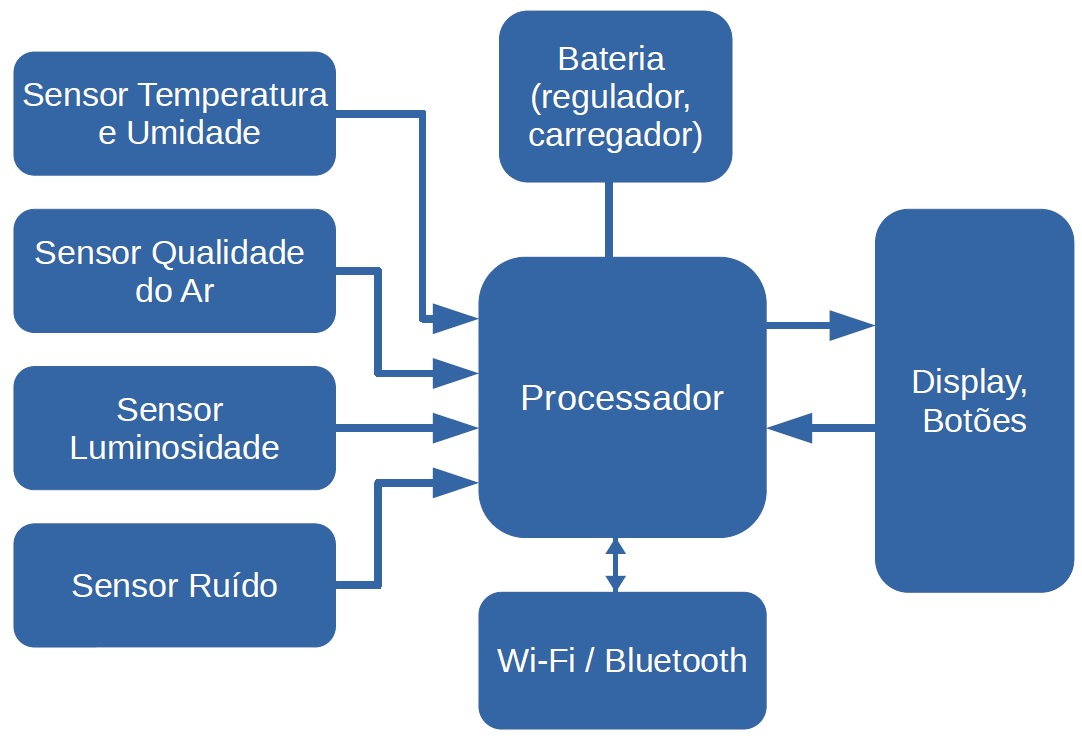
\includegraphics[width=10cm]{block_diagram}
    \caption{Diagrama de Blocos simplificado do dispositivo}
    \label{fig:Diagrama de Blocos}
\end{figure}

\subsubsection{Sensores}
A fim de atender aos critérios apresentados para o monitoramento, foram escolhidos os seguintes sensores: 
\begin{itemize}
\item \textbf{AS7262}\cite{as7262}, da AMS: 

Atende aos requisitos de medição de \textit{conforto luminoso}. 

\textbf{Medidas}: Intensidade e cor da luz incidente.

A cor da luz, nesse sensor, é medida através de 6 canais, correspondendo aos espectros de luz vermelha (650nm), laranja (600nm), amarela (570nm), verde (550nm), azul (500nm) e violeta (450nm), ao invés de simples RGB, com resolução de 16 bits.

\textbf{Comunicação}: I²C, SPI ou UART (configurável)

\item \textbf{BME280} \cite{bme280}, da Bosch: 

Atende aos requisitos de \textit{conforto térmico}. 

\textbf{Medidas}: 
    \begin{itemize}
    \item Temperatura entre -40 e 85°C, com precisão de ±1.0°C
    \item Umidade relativa com precisão de ±3\%
    \item Pressão entre 300 e 1100hPa, com precisão ±1 hPa
    \end{itemize}

\textbf{Comunicação}: SPI ou I²C

\item \textbf{SGP30} \cite{sgp30}:

Sensor para medições de aplicação \textit{indoor}. 

\textbf{Medidas}:
    \begin{itemize}
    \item TVOC entre 0 ppb e 60000 ppb, com resolução de 1ppb
    \item $CO_{2}$ entre 400 ppm e 60000 ppm, com resolução de 1ppb
    \end{itemize}

\textbf{Comunicação}: I²C

\item \textbf{Microfone de Eletreto}:

Em conjunto com um circuito amplificador, atende aos requisitos de \textit{conforto acústico}. 

\textbf{Medida}: volume de ruído sonoro ambiente

\textbf{Comunicação}: Analógica, precisão de 12 bits (resolução do conversor analógico-digital do ESP32). 
\end{itemize}

\subsubsection{Feedback}

Para Sistema de coleta de \textit{feedback} nos dispositivos, optamos por utilizar um display OLED\cite{oled} de 128x64 pixels, com driver de comunicação I2C, e 2 botões do tipo \textit{push button}. 

\subsubsection{Processador}

De acordo com a mesma pesquisa da Aspencore citada anteriormente, 61\% dos projetos de sistemas embarcados usam processadores de 32-bits, e 65\% utiliza algum tipo de sistema operacional. 

A partir das especificações dadas, listamos os periféricos necessários ao microcontrolador, e buscamos as principais opções existentes no mercado para atuar como processador central do dispositivo. 

Como a comunicação dos dispositivos é uma funcionalidade crucial, foi dada a preferência para os \textit{System-on-a-Chip} (SoCs), ou Sistema em um chip, ao invés de microcontroladores e módulos \textit{wireless} independentes. SoC é o nome dado a circuitos integrados que englobam processadores (ou microcontroladores, usualmente em dispositivos embarcados), memórias, dentre outros módulos, como circuitos para comunicação sem fio, personalizados para uma aplicação \cite{soc}. Assim, chegamos a três opções de SoCs com \textbf{bluetooth} integrado. 


\begin{center}
\begin{table}
\begin{tabular}{|c|c|c|c|c|} 
\hline
\textbf{Vendor} & \textbf{Chip} & \textbf{Price} & \textbf{Kit} & \textbf{Kit Price} \\
\hline
Nordic Semi & BMD350 & \$11.3 & BMD350-EVAL & \$89 \\ 
Espressif Systems & ESP32 & \$3.8 & ESP32-DevKitC & \$10 \\ 
STMicroelectronics & BlueNRG-2 & \$3.5 & BlueNRG-Tile & \$50 \\ 
\hline
\end{tabular}
\caption{Tabela comparativa de processadores}
\label{table}
\end{table}
\end{center}

Analisando principalmente os ambientes de desenvolvimento, a documentação disponível e o preço dos CIs e de seus kits de desenvolvimento, optamos pela família ESP32 \cite{ESP32}. 

Além do Wi-fi como diferencial no SoC, a Espressif possui um bom suporte e ferramentas de desenvolvimento focadas em BLE e Wi-Fi, em especial para o uso de BLE Mesh, e um dos menores preços, assim considerado o melhor custo-benefício. 

\textbf{Especificações do ESP32:} \cite{ESP-datasheet}
\begin{itemize}
\item \textbf{Processador}: Xtensa 32-bits, dual core
\item \textbf{Wi-Fi}: 802.11 b/g/n
\item \textbf{Bluetooth}: v4.2 BR/EDR e BLE
\end{itemize}



\subsubsection{Alimentação}

Para alimentar os dispositivos, foi pensado inicialmente em utilizar uma bateria recarregável, de forma que o dispositivo seja portátil e não necessite da rede elétrica para funcionar. A tensão da bateria seria então regulada para 3.3V a fim de alimentar todos os circuitos da placa, que operam nessa tensão. 

Com um conector USB e um circuito apropriado integrado na placa, seria possível recarregar a bateria sem interromper o funcionamento do dispositivo. Para fins de teste, como a placa de desenvolvimento ESP32 possui um USB micro e um regulador de 3.3V, optamos por utilizá-lo como alimentação para os demais módulos. Os dispositivos ficam, assim, conectados ao computador ou a tomada durante os testes.

\subsection{Protocolos de Comunicação e Arquitetura da Rede}

Os dispositivos serão interconectados por meio de uma rede \textit{Bluetooth Mesh}, disponibilizando dados de medições dos sensores e \textit{feedback} ao longo do dia por toda a rede. Essa arquitetura utiliza o conceito de rede por inundação, no qual os dados de um nó são enviados para vários outros nós, que atuam como retransmissores desses dados para outros dispositivos dentro do seu alcance, o que aumenta a área de cobertura da rede e sua confiabilidade, já que se um dos dispositivos se desconectar, outras rotas estarão disponíveis para a propagação dos dados.

Apenas um dos dispositivos da rede estará conectado também à Internet via Wi-Fi, atuando como um gateway para a rede, sendo assim necessário que este também esteja conectado a uma fonte fixa de energia. Essa conexão permitirá o envio dos dados coletados pela rede para um servidor externo ao sistema, possibilitando o acesso remoto aos dados.

O artigo \cite{analise-protocolos-iot} faz uma comparação dos protocolos mais utilizados em aplicações IoT, citados na seção \ref{protocolos-aplicacao}, de maneira prática, utilizando um \textit{testbed} muito parecido com o que utilizamos para o desenvolvimento desse projeto - microcontrolador ESP8266 ao invés do ESP32. A partir das conclusões presentes no artigo, podemos ver que o protocolo MQTT se mostrou mais estável em relação ao CoAP ao utilizar esse dispositivo restrito, aguentando maior carga de dados e maior confiabilidade na entrega dos mesmos, o que o torna ideal para a aplicação desse projeto.

%> OBS: inserir imagem da arquitetura da rede 

\subsection{Software}

%*MQTT broker (necessidade + descr)
O uso do protocolo MQTT na rede de dipositivos torna necessária a implementação de um \textit{MQTT Broker} para a recepção dos dados coletados. Utilizamos o Eclipse Mosquitto \cite{mosquitto}, uma implementação de código aberto disponibilizada pela Eclipse Foundation, bastante utilizado em projetos que usam essa tecnologia.  
%* Telegraf (necessidade + descr)
%* InfluxDB (descr)
%* Grafana (descr)
%* AWS (descr)

%> Falar de nuvem no final, reforçando a ideia que foi passada nos requisitos, e linkar o geral com a imagem final


\end{document}
